\begin{figure}%
  \def\frac{0.24}
  \rotatebox{90}{\hspace{2em}\color{blue}{\tiny Fetch Reach}}%
  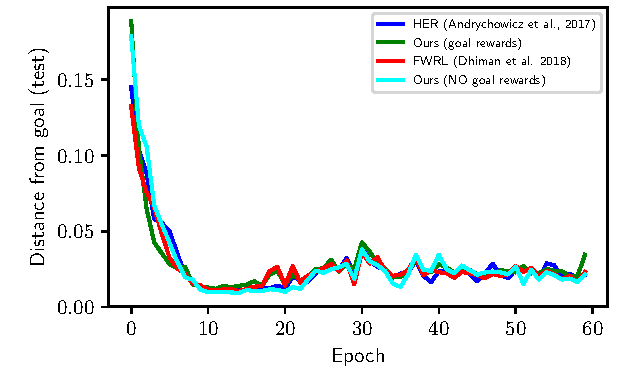
\includegraphics[width=\frac\columnwidth]{media/res/6efc1de-path_reward_low_thresh_chosen-FetchReachPR-v1-dqst/epoch-test/ag_g_dist.pdf}%
  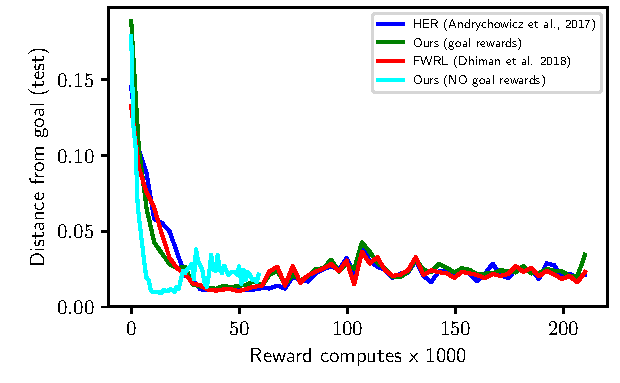
\includegraphics[width=\frac\columnwidth]{media/res/6efc1de-path_reward_low_thresh_chosen-FetchReachPR-v1-dqst/reward_computes-test/ag_g_dist.pdf}%
  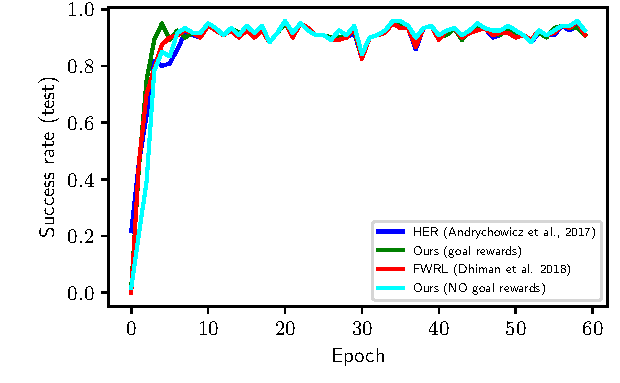
\includegraphics[width=\frac\columnwidth]{media/res/6efc1de-path_reward_low_thresh_chosen-FetchReachPR-v1-dqst/epoch-test/success_rate.pdf}%
  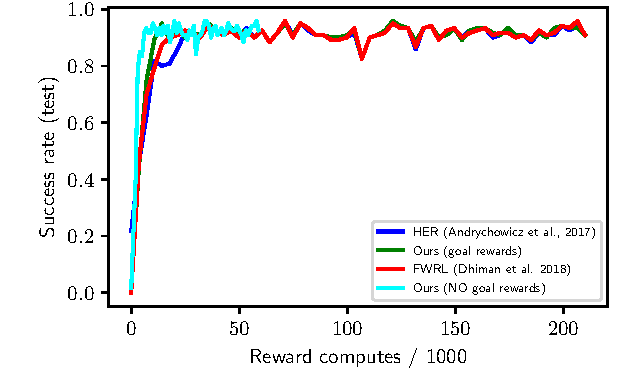
\includegraphics[width=\frac\columnwidth]{media/res/6efc1de-path_reward_low_thresh_chosen-FetchReachPR-v1-dqst/reward_computes-test/success_rate.pdf}\\
  \rotatebox{90}{\hspace{2em}\color{blue}{\tiny Fetch Push}}%
  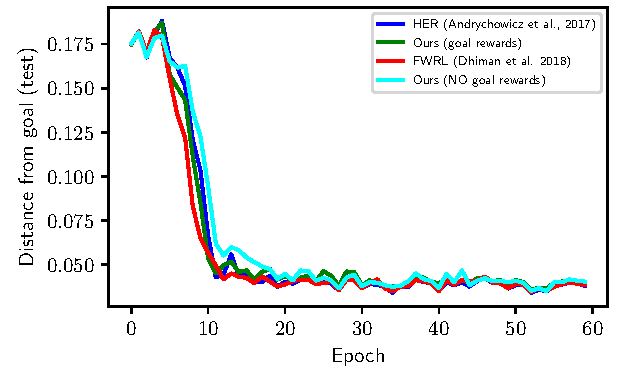
\includegraphics[width=\frac\columnwidth]{media/res/6efc1de-path_reward_low_thresh_chosen-FetchPushPR-v1-dqst/epoch-test/ag_g_dist.pdf}%
  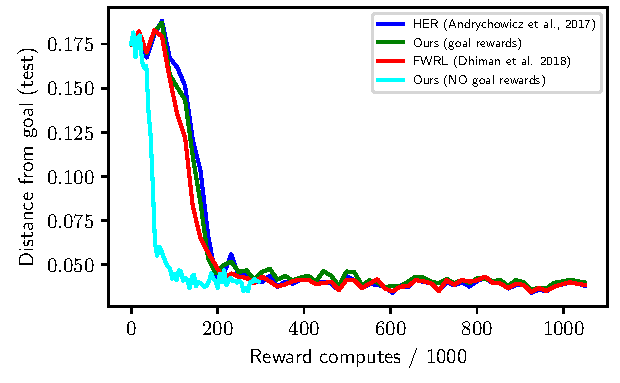
\includegraphics[width=\frac\columnwidth]{media/res/6efc1de-path_reward_low_thresh_chosen-FetchPushPR-v1-dqst/reward_computes-test/ag_g_dist.pdf}%
  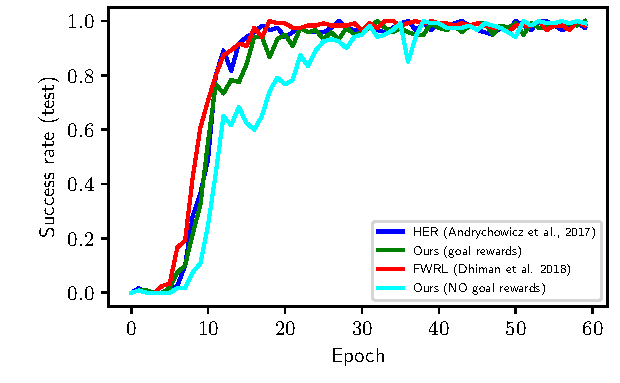
\includegraphics[width=\frac\columnwidth]{media/res/6efc1de-path_reward_low_thresh_chosen-FetchPushPR-v1-dqst/epoch-test/success_rate.pdf}%
  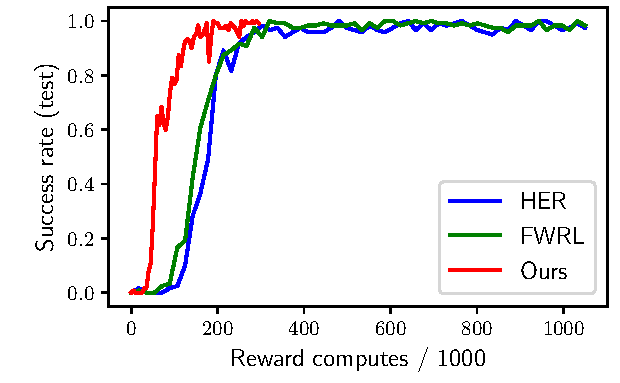
\includegraphics[width=\frac\columnwidth]{media/res/6efc1de-path_reward_low_thresh_chosen-FetchPushPR-v1-dqst/reward_computes-test/success_rate.pdf}\\
  \rotatebox{90}{{\tiny\hspace{1em} \color{blue}{Fetch Pick And Place}}}%
  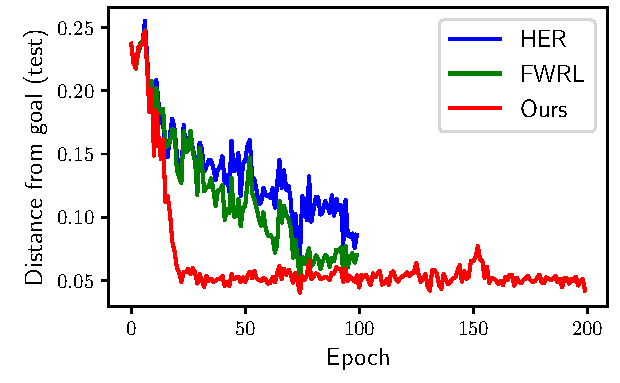
\includegraphics[width=\frac\columnwidth]{media/res/6efc1de-path_reward_low_thresh_chosen-FetchPickAndPlacePR-v1-dqst/epoch-test/ag_g_dist.pdf}
  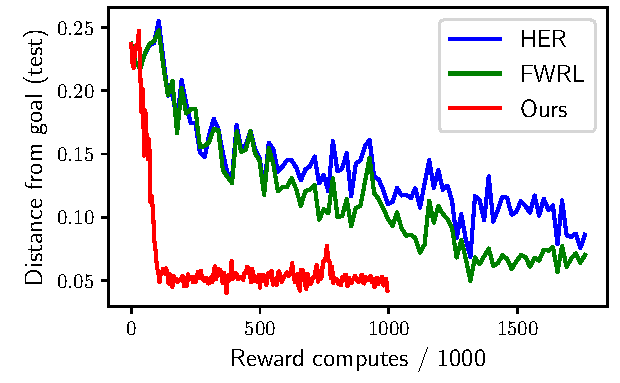
\includegraphics[width=\frac\columnwidth]{media/res/6efc1de-path_reward_low_thresh_chosen-FetchPickAndPlacePR-v1-dqst/reward_computes-test/ag_g_dist.pdf}%
  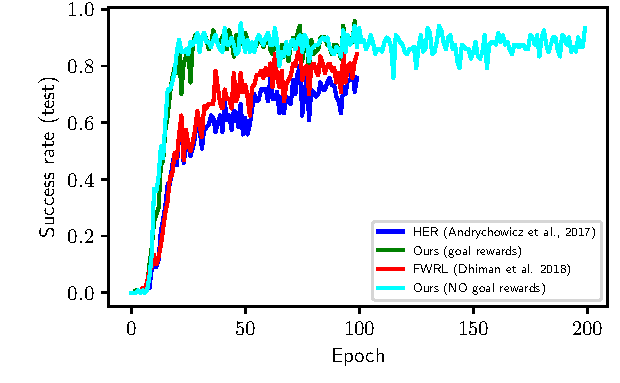
\includegraphics[width=\frac\columnwidth]{media/res/6efc1de-path_reward_low_thresh_chosen-FetchPickAndPlacePR-v1-dqst/epoch-test/success_rate.pdf}%
  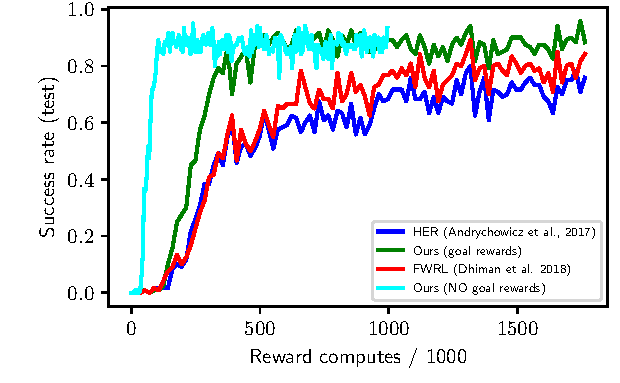
\includegraphics[width=\frac\columnwidth]{media/res/6efc1de-path_reward_low_thresh_chosen-FetchPickAndPlacePR-v1-dqst/reward_computes-test/success_rate.pdf}\\
  \rotatebox{90}{\tiny\hspace{2em}\color{blue}{Fetch Slide}}%
  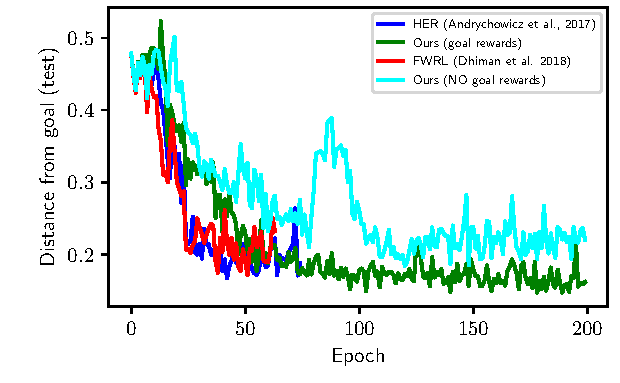
\includegraphics[width=\frac\columnwidth]{media/res/6efc1de-path_reward_low_thresh_chosen-FetchSlidePR-v1-dqst/epoch-test/ag_g_dist.pdf}
  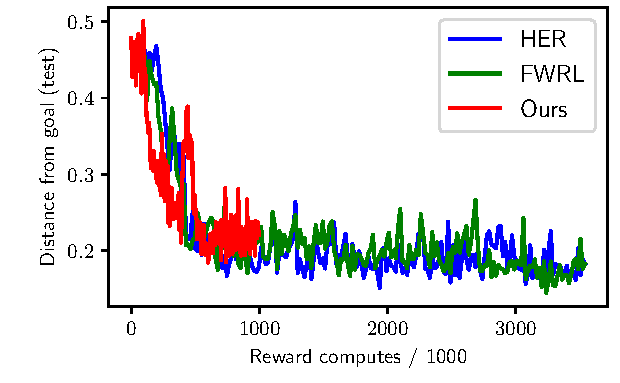
\includegraphics[width=\frac\columnwidth]{media/res/6efc1de-path_reward_low_thresh_chosen-FetchSlidePR-v1-dqst/reward_computes-test/ag_g_dist.pdf}%
  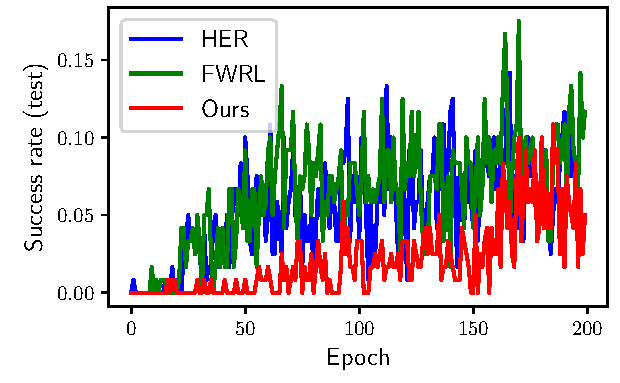
\includegraphics[width=\frac\columnwidth]{media/res/6efc1de-path_reward_low_thresh_chosen-FetchSlidePR-v1-dqst/epoch-test/success_rate.pdf}%
  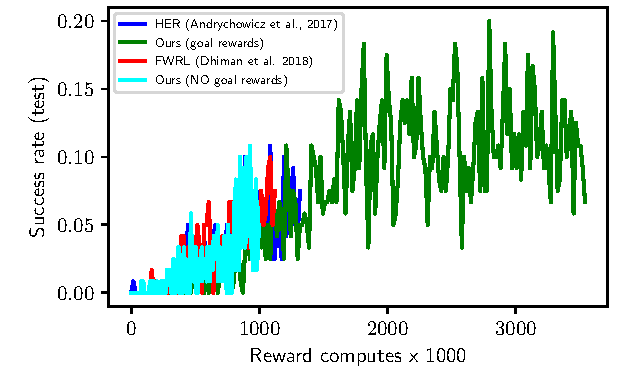
\includegraphics[width=\frac\columnwidth]{media/res/6efc1de-path_reward_low_thresh_chosen-FetchSlidePR-v1-dqst/reward_computes-test/success_rate.pdf}\\
  {.\tiny\color{blue}\hspace{0.8cm}(a) Distance on Epochs \hspace{1.05cm}(b) Distance on
    reward computes
    \hspace{0.70cm} (c) Success rate on epochs \hspace{0.9cm} (d) Success rate on reward computes}
  \caption{We compare our method against HER~\citep{andrychowicz2016learning}
    and FWRL~\citep{dhiman2018floydwarshall} and get comparable performance for
    Fetch Reach and Push tasks. For Pick and Place task, our method works the
    best, while for Slide task baselines are better.
    When the number of reward computations is take into account our method learns
    much faster than across all tasks.}%
  \label{fig:fetch-results}%
\end{figure}
